\chapter[从个人到团队]{锻炼高效: 从个人到团队} 

个人精力有限,必须借用团队才能成倍提高生产率。但不能仅靠组长个人的努力:例如有些开发技术出身的组长,自我时间控制很好,技术也不错,但不懂如何有效下放工作,协助团队成员,导致团队不懂,做不出来,最后组长就自己动手搞定,恶性循环。
所以团队要有效率,除了依赖个人能力外,还需要了解高效团队的挑战。

\framebox{%
\begin{minipage}[t]{0.97\columnwidth}\raggedright
知识工厂 (Knowledge Factory)

一位老同学在东莞有一个"知识工厂",主要是为美国客户服务,输入扫描件,输出修正好的、正确的英文文件。\\
因为美国的人工费用很高,所以客户愿意把一些耗费人力的手工工作外包。\\
虽然公司可以利用识别英文字的软件把扫描件转化成电子版,但只能做到大部分,还是有很多地方需要看原文,手工输入、修正。这个知识工厂就是找一些初中学历的人,经过简单培训后上岗,把编辑好的文档发回给美国客户。一般是按字数收钱,因为是外包业务,利润非常低,所以必须要控制生产效率------如果效率低工厂就不赚钱了。但效率不仅仅是速度,如果有太多错误,客户便不满意,所以也要控制质量。\\
\textbf{典型客户}:\\
*某网站服务,收集了大量老资料,专门帮助美国人寻根。

\begin{itemize}
\tightlist
\item
  例如某美国人可能前几代是从爱尔兰过来,但只知道是哪年哪月,他可以从这网站搜索某时间段轮船的客户名单,所以这公司便需要把大量老轮船客户名单,转换成电子文件,其中也会遇到很多古老的字,扫描软件难以识别。
\end{itemize}

有一天他邀请我去参观东莞分厂,办公大厅里有很多人,大家头戴耳机在屏幕前敲打键盘。\\
员工每 7 - 10
人分成一个小组,每组一个组长,每组头上有个大屏幕,显示着数字。\\
我就问同学这是干什么的,他说这些就是反应每个小组当前的速度,每个组员都可以看到,效果就是让成员们能直观看到工作的反馈:现在整个组的速度、质量如何,都可以从那些数字简单地反映出来。\\
我老同学说:\\
``每个员工和团队都很清楚当前的效率和质量。
从这么多年数据显示,一般新员工经过培训后开始 1 分钟是 55- 85 WPM(Word
per Minute )。
但因为经验少,所以一般错误率比较高。经过几个月的实际工作,速度和准确率都会有提升。我们提拔组长也主要是看他过去的指标是否领先。\\
除了监控,我们也会完善一下新的系统来帮助团队,例如,系统会同步给他们一些提示,也会用语英语读出来,帮助他们更好完成任务。``\\
\strut
\end{minipage}}

以上是团队如何利用系统,提高生产率和质量,让公司盈利生存的例子。
我立马想到,如果没有及时的数字反馈,很难让团队知道自己现在的状态。这跟我每天早上跑步一样,如果没有计时,就没有动力保持或超越以前的速度。\\
克服拖延症里面提过的效率小手册第二章里的“做事要有条理” (Becoming Organized)
如果个人无法把所有所做的事情清晰地分解,就很难有效率。比如,小手册提了几点简单的组织系统帮我们:

\begin{enumerate}
\tightlist
\item
  分成项目 (20 Projects)
\item
  项目由任务组成 (21 Tasks)
\item
  任务或活动,要有开始日期,结束日期 (22 Events)
\item
  分支法 (24 Branch)
\end{enumerate}

一个人要管理一个团队,当那些任务不是仅仅是自己看和做,而是要分摊到团队其他人去完成的时候,就更需要有个系统,让大家看到计划与实际。在项目管理来讲,这个叫工作任务分解
(Work Breakdown Structure WBS)。

我在北京给一家公司做评审时,问他怎么管理项目,他很自信的说跟你上次见不一样了,我们现在有项目管理系统。

其实他说的管理系统只是一个任务管理系统(类似缺陷管理,每一个缺陷或任务独立,然后就让成员填写任务的完成情况)。因为系统只能跟踪任务的实际完成情况,没有WBS分解能力,难以管理整个项目。可以想象,如果项目有一百多个任务,经理怎么知道任务的进展情况呢?只能看到每个任务状态。但是如果能把任务按过程(如测试,编码),模块(如
A模块、B模块等)或迭代分组,我就可以把那100多个任务汇总成5、6个组,经理或团员就可以从系统中得知项目的情况。

:= = = = =\\

某家做保险系统的国际公司,因为要控制人手,所以采用了外包模式,让顾问公司提供人员来现场做开发,公司内的项目经理手下可能有五、六十人在工作。
以前,他要监控这些开发活动时,需要去检查每个人的情况,忙不过来。
这就可以用一个 WBS 管理的系统,来全局监控开发的情况。
WBS项目管理系统如何帮到这个项目经理呢?
项目管理系统要求每个任务(或工作包)都需要有产出物,而且产出物必须通过评审才算百分之百完成。这样的话项目经理就不需要逐个产出物自己查看了,他可以安排团队自己相互评审产出物,项目经理就可以总体监控项目进展,提高团队效率。\\

:= = = = = =

有些高层也了解项目管理有不足,但觉得是流程的问题,要求先把流程建好,才上自动化系统。这种思路听起来很有道理,但实际上行不通。

原因是过程跟系统是息息相关的,如果没有系统,你的过程只是基于一堆手工模板,无法操作,就好比你可以用excel表希望做项目管理系统一样。原因是那些excel表它不是一个系统,最大的问题是它可以随时更改结果,所以这种系统出来的报告,都是说没有偏差。对监控项目没有作用。
我们后面就用一个实例看看怎么在开始的时候可以尽快尝试一下怎么用一些系统来帮我们管理个人的小项目,因为我们说所有过程改进都应该先从小的试点开始。

现在我们都流行用SaaS系统(Software as a
Service),所以很多服务都可以在线上直接使用,不需要预先安装服务器,数据库,应用软件,配置等等。比如我随便进一个这类的WBS项目管理系统,我输入这两周主要的一些主要活动,如:

\begin{itemize}
\tightlist
\item
  用水晶球完善预测模型
\item
  完善国际功能点教材与资料
\item
  为简化功能点准备一套资料,让公司可以开始使用
\end{itemize}


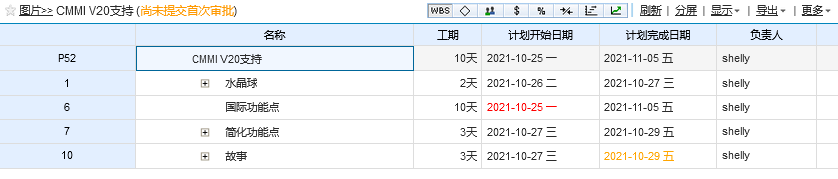
\includegraphics[width=10cm]{微信截图_20211029132308.jpg}

因为我都在外面忙,我只是可以把这些重点设出来。然后每天会议要求做的人在里面添加活动:

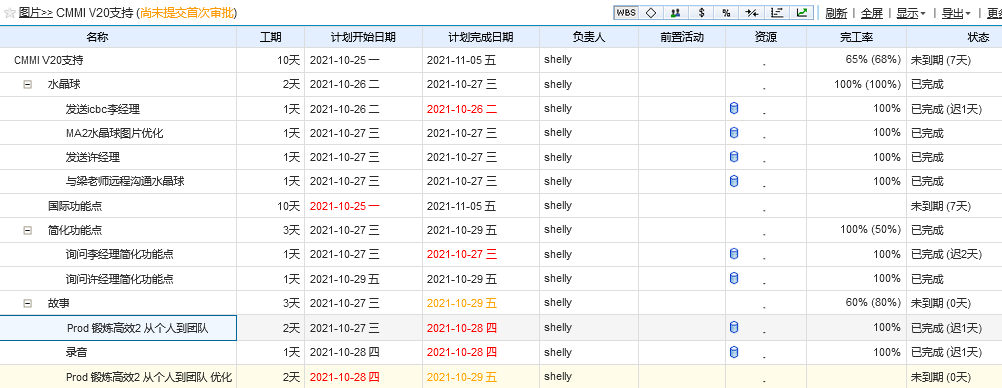
\includegraphics[width=10cm]{微信截图_20211029090316.jpg}

因为它是一个SaaS系统,所有团队的成员不一定是在同一个办公地点,都可以看到,还可以上传任务的产出物,并看到任务的完成百分比。

每周五,各人在系统填写实际工时(注意:在她填写实际工时的时候,能看到每活动的计划工时):


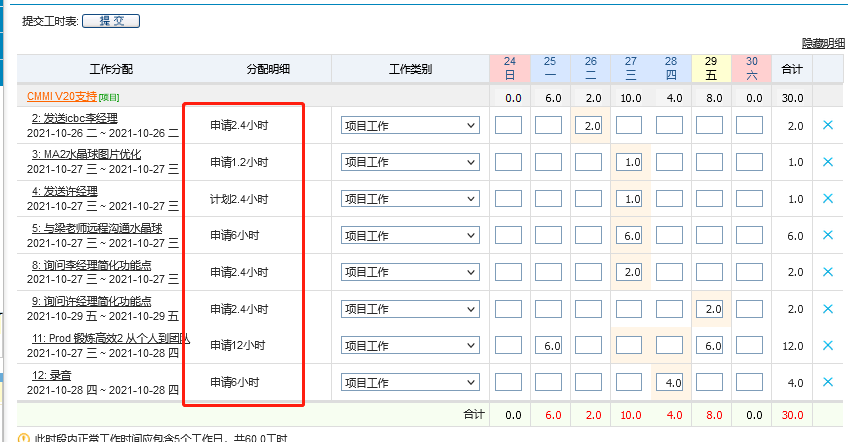
\includegraphics[width=10cm]{微信截图_20211029090520.jpg}

在没有做这个之前,我也尝试过在大白纸上面每人写上当天和每周的活动,要团队每天下班拍照发我,但发现一点用都没有:

\begin{enumerate}
\tightlist
\item
  我没时间去看里面有没有具体的时间、工作量
\item
  缺乏数字性记录
\end{enumerate}

我开始用这个系统后,两个月过去,就可以有一些统计数据,从系统里面可以抓出来团队或者个人在过去这个时间完成了什么任务,因为都在系统有记录,也因为有产出物,我用Wiki
跟踪这些产出物的话,我就可以在 Wiki
里面记录每一个产出物的缺陷,所以也可以得到每个人或者团队的质量。把本来只是我个人的管理,扩大到团队管理。


